\documentclass[a4paper,10pt]{article}
\usepackage[T1]{fontenc}\usepackage{amsmath}\usepackage{txfonts}\usepackage{booktabs}\usepackage{graphicx}\usepackage{natbib}\usepackage{xr}\externaldocument{../paper/Ramteke_2026_substructure_stress_test}
\usepackage[margin=2cm]{geometry}\usepackage{caption}
\renewcommand{\thetable}{S\arabic{table}}\renewcommand{\thefigure}{S\arabic{figure}}
\newcommand{\Msun}{M_\odot}
\newcommand{\thetaE}{\theta_{\rm E}}
\newcommand{\dchi}{\Delta\chi^2}
\newcommand{\dpsi}{$\delta\psi$}
\newcommand{\TODO}[1]{\textcolor{red}{[#1]}}
\renewcommand{\topfraction}{0.9}\renewcommand{\bottomfraction}{0.8}\renewcommand{\textfraction}{0.07}
\renewcommand{\floatpagefraction}{0.75}\renewcommand{\dbltopfraction}{0.9}\renewcommand{\dblfloatpagefraction}{0.75}
\begin{document}
\begin{center}{\Large\bfseries Supplementary tables and figures}\\[4pt]
\emph{Stress-testing dark-matter substructure detectors on a common simulation suite}\\ R. Ramteke, submitted to A\&A (AA63827-26)\end{center}
\noindent These tables and figures are cited from the paper as supplementary Tables S1--S15 and Figs.~S1--S3. Section, table and figure numbers inside the captions refer to the paper.

\begin{table}[!htbp]
\caption{Threshold-free comparison. Area under the ROC curve against the clean control, and completeness at 10\% and 1\% false-positive rate, on the common set of Table~\ref{tab:fullpop}, each threshold set on the 1\,000-lens clean control; Table~\ref{tab:lowfpr} gives the 1\% values on the larger clean controls. The common set excludes the most massive lenses, which lowers the U-Net's AUC (0.62 here, 0.67 on all lenses). The U-Net is the mean of four seeds.}
\label{tab:roc}
\centering
\scriptsize
\setlength{\tabcolsep}{3pt}
\begin{tabular}{@{}llccc@{}}
\toprule
family & population & AUC & TPR at 10\% FPR & TPR at 1\% FPR \\
\midrule
A joint scan & $c{=}60$ & 0.921 & 85\% & 78\% \\
 & $c{=}15$ & 0.908 & 81\% & 76\% \\
 & multipole & 0.975 & 98\% & 97\% \\
\addlinespace[2pt]
B free-form residual & $c{=}60$ & 0.751 & 53\% & 16\% \\
 & $c{=}15$ & 0.683 & 38\% & 2\% \\
 & multipole & 0.897 & 70\% & 2\% \\
\addlinespace[2pt]
C U-Net & $c{=}60$ & 0.620 & 32\% & 21\% \\
 & $c{=}15$ & 0.517 & 12\% & 3\% \\
 & multipole & 0.504 & 10\% & 2\% \\
\addlinespace[2pt]
\bottomrule
\end{tabular}

\end{table}

\clearpage

\begin{table}[!htbp]
\caption{Family~A, the joint scan, at three operating points on the full 1\,000-lens Tier-0 populations. Completeness on retained fits; the paired flip counts the 831 lenses both concentration scans retain; the mass error of the localized detections agrees with that of all detections to within 0.02~dex.}
\label{tab:joint_ops}
\centering
\scriptsize
\setlength{\tabcolsep}{3pt}
\begin{tabular}{@{}lccc@{}}
\toprule
 & 10\% FPR & $\dchi\ge20$ & $\dchi\ge100$ \\
\midrule
threshold on $\dchi$ & $6.3$ & $20.0$ & $100.0$ \\
FPR, clean & 10.0\% & 0.20\% & 0.20\% \\
FPR, multipole $a_4{=}0.01\,\thetaE$ & 97\% & 86\% & 47\% \\
FPR, multipole $a_4{=}0.03\,\thetaE$ & 97\% & 96\% & 90\% \\
FPR, multipole $a_3{=}0.03\,\thetaE$ & 98\% & 98\% & 96\% \\
\addlinespace[2pt]
compl.\ $c{=}60$, $10^{9.0}$--$10^{9.5}\Msun$ & 98\% & 93\% & 60\% \\
compl.\ $c{=}60$, $10^{9.5}$--$10^{10.0}\Msun$ & 99\% & 95\% & 87\% \\
compl.\ $c{=}60$, $10^{10.0}$--$10^{10.5}\Msun$ & 96\% & 96\% & 94\% \\
compl.\ $c{=}60$, $10^{10.5}$--$10^{11.0}\Msun$ & 97\% & 97\% & 97\% \\
compl.\ $c{=}15$, $10^{9.0}$--$10^{9.5}\Msun$ & 95\% & 82\% & 41\% \\
compl.\ $c{=}15$, $10^{9.5}$--$10^{10.0}\Msun$ & 95\% & 92\% & 77\% \\
compl.\ $c{=}15$, $10^{10.0}$--$10^{10.5}\Msun$ & 95\% & 94\% & 89\% \\
compl.\ $c{=}15$, $10^{10.5}$--$10^{11.0}\Msun$ & 97\% & 97\% & 94\% \\
paired flip $c{=}60\to15$, lost\,:\,gained & 68\,:\,32 & 47\,:\,9 & 67\,:\,5 \\
\addlinespace[2pt]
detections of $c{=}60$ subhalos & 710 & 603 & 475 \\
localized ($\le2$ px) & 19.9\% & 20.7\% & 21.1\% \\
mass error, all detections (dex) & $+0.39$ & $+0.42$ & $+0.48$ \\
\bottomrule
\end{tabular}

\end{table}

\clearpage

\begin{table}[!htbp]
\caption{The same lenses at three depths, everything else identical. The joint scan is calibrated on the clean control of its own variant (deep: full populations; 600~s: 200-lens subsamples; shallow: 300-lens subsamples). The U-Net trained deep is scored at its deep threshold and recalibrated on each variant's control; a second set is retrained on 30\,000 shallow images. $^{a}$Four bins, $10^{9}$--$10^{9.5}$ / $10^{9.5}$--$10^{10}$ / $10^{10}$--$10^{10.5}$ / $10^{10.5}$--$10^{11}\,\Msun$, in per cent. $^{b}$Median over the $c=60$ population of $[\sum_{\rm pix}(I_{\rm noiseless}/\sigma)^2]^{1/2}$.}
\label{tab:depth}
\centering
\scriptsize
\setlength{\tabcolsep}{2.5pt}
\begin{tabular}{@{}lccc@{}}
\toprule
 & deep & 600 s & shallow \\
exposure time & 5400 s & 600 s & 135 s \\
median arc S/N$^{b}$ & $1.5\times10^{3}$ & $4.9\times10^{2}$ & $2.2\times10^{2}$ \\
median peak-pixel S/N & 235 & 78 & 37 \\
\midrule
\multicolumn{4}{@{}l}{\emph{A, joint scan}} \\
\quad threshold at 10\% FPR & $6.3$ & $5.8$ & $6.7$ \\
\quad clean FPR at $\dchi\ge20$ & 0.20\% & 0.00\% & 1.00\% \\
\quad macro fits rejected, $c{=}60$ & 70/1000 & 2/200 & 0/300 \\
\quad compl.\ $c{=}60$, 10\% cal.$^{a}$ & 98 / 99 / 96 / 97 & 76 / 96 / 95 / 93 & 59 / 84 / 89 / 92 \\
\quad compl.\ $c{=}60$, 10\% cal., 8--8.5 / 8.5--9 & 47 / 79 & -- & 8 / 9 \\
\quad compl.\ $c{=}60$, $\dchi\ge20$$^{a}$ & 93 / 95 / 96 / 97 & 52 / 89 / 93 / 93 & 16 / 63 / 81 / 90 \\
\quad compl.\ $c{=}15$, $\dchi\ge20$$^{a}$ & 82 / 92 / 94 / 97 & -- & 6 / 37 / 58 / 88 \\
\quad FPR multipole, cal.\ / $\ge20$ & 97\% / 96\% & -- & 83\% / 57\% \\
\addlinespace[2pt]
\multicolumn{4}{@{}l}{\emph{C, U-Net trained deep (4 seeds)}} \\
\quad clean FPR at deep threshold & 10\% & 79\% & 88\% \\
\quad AUC, $c{=}60$ vs.\ clean & 0.67 & 0.58 & 0.52 \\
\quad compl.\ $c{=}60$, recal.\ 10\%$^{a}$ & 19 / 51 / 70 / 79 & 12 / 16 / 32 / 40 & 9 / 11 / 12 / 17 \\
\addlinespace[2pt]
\multicolumn{4}{@{}l}{\emph{C, U-Net retrained on 30\,000 shallow images (2 seeds)}} \\
\quad AUC, $c{=}60$ vs.\ clean & -- & -- & 0.57 \\
\quad compl.\ $c{=}60$$^{a}$ & -- & -- & 14 / 19 / 34 / 53 \\
\quad compl.\ $c{=}15$$^{a}$ & -- & -- & 12 / 12 / 12 / 13 \\
\bottomrule
\end{tabular}

\end{table}

\clearpage

\begin{table}[!htbp]
\caption{Lens light added and subtracted two ways, 300 lenses per population (joint scan on the first 200), $c=15$ template; fits with $\chi^2/{\rm dof}\ge10$ excluded. ``None'': Tier~0 without lens light. ``Single'': one S\'ersic fitted to the two-component truth; ``double'': the correctly specified fit. S1 and S2 are two independent 300-lens seed sets; the joint scan and the free-form statistic are run on S1 only. The U-Net is the four-seed mean on each set.}
\label{tab:lenslight}
\centering
\footnotesize
\setlength{\tabcolsep}{5pt}
\begin{tabular}{@{}lccccc@{}}
\toprule
 & none & \multicolumn{2}{c}{single} & \multicolumn{2}{c}{double} \\
 & & S1 & S2 & S1 & S2 \\
\midrule
\multicolumn{6}{@{}l}{\emph{smooth fit of the fixed-macro scan (shared with B)}} \\
clean fits rejected (of 300) & 5 & 141 & 148 & 21 & 12 \\
\multicolumn{6}{@{}l}{\emph{A, joint scan (first seed set, 200 lenses; ``none'': full 1\,000-lens populations)}} \\
\quad threshold, 10\% FPR ($\dchi$) & 6.3 & 1179 & -- & 6.2 & -- \\
\quad FPR clean, $\dchi\ge20$ / $\ge100$ & 0.20 / 0.20\% & 97 / 88\% & -- & 0.51 / 0.51\% & -- \\
\quad FPR multipole, $\dchi\ge20$ / $\ge100$ & 96 / 90\% & 99 / 98\% & -- & 97 / 85\% & -- \\
\quad compl.\ $10^{9.5}$--$10^{10}\Msun$, 10\% cal.\ & 99\% & 58\% & -- & 96\% & -- \\
\quad compl.\ $10^{10}$--$10^{10.5}\Msun$, 10\% cal.\ & 96\% & 100\% & -- & 97\% & -- \\
\multicolumn{6}{@{}l}{\emph{A, fixed-macro scan (Appendix C)}} \\
\quad threshold, 10\% FPR ($\dchi$) & $-10.6$ & $+86$ & $+99$ & $-7.5$ & $-9.3$ \\
\quad FPR clean, $\dchi{>}20$ / ${>}100$ & 0.68 / 0\% & 25 / 9\% & 26 / 10\% & 0 / 0\% & 0.35 / 0\% \\
\quad compl.\ $10^{10}$--$10^{10.5}\Msun$ & 85\% & 53\% & 64\% & 79\% & 89\% \\
\multicolumn{6}{@{}l}{\emph{B, free-form residual statistic}} \\
\quad threshold, $\max|\delta\kappa|$ & 0.10 & 0.96 & -- & 0.09 & -- \\
\quad compl.\ $10^{10}$--$10^{10.5}\Msun$ & 92\% & 12\% & -- & 98\% & -- \\
\multicolumn{6}{@{}l}{\emph{C, U-Net (four seeds), on the subtracted images}} \\
\quad AUC ($c{=}60$ vs.\ clean) & 0.67 & 0.58 & 0.57 & 0.67 & 0.66 \\
\quad FPR clean at Tier-0 thr.\ & 10\% & 78\% & 80\% & 47\% & 49\% \\
\quad compl.\ $10^{10}$--$10^{10.5}\Msun$, recal.\ & 70\% & 24\% & 28\% & 56\% & 60\% \\
\bottomrule
\end{tabular}

\end{table}

\clearpage

\begin{table}[!htbp]
\caption{$c=60$ completeness (\%) at each family's own 10\% threshold on the full population, counting all detections and only those whose reported position lies within 2~pixels ($0.16''$) of the subhalo.}
\label{tab:loccomp}
\centering
\footnotesize
\begin{tabular}{@{}lcccccc@{}}
\toprule
 & \multicolumn{6}{c}{$c=60$ completeness (\%): all detections / localized only} \\
family & 8--8.5 & 8.5--9 & 9--9.5 & 9.5--10 & 10--10.5 & 10.5--11 \\
\midrule
A grid scan & 47 / 11 & 79 / 18 & 98 / 20 & 99 / 13 & 96 / 17 & 97 / 24 \\
A position-free scan & 50 / 37 & 79 / 70 & 98 / 90 & 99 / 96 & 96 / 92 & 99 / 93 \\
B free-form & 15 / 0 & 12 / 3 & 45 / 31 & 87 / 73 & 96 / 66 & 97 / 58 \\
C U-Net, 30\,000 & 11 / 0 & 11 / 0 & 21 / 10 & 49 / 45 & 69 / 66 & 78 / 77 \\
C U-Net, $5\times10^{5}$ & 9 / 2 & 17 / 9 & 38 / 32 & 74 / 71 & 84 / 84 & 92 / 90 \\
\bottomrule
\end{tabular}

\end{table}

\clearpage

\begin{table}[!htbp]
\caption{Localization on the same lenses: the 726 $c=60$ lenses that Families A and B both retain, each family at its own 10\% threshold. Per cent of detections within 2~pixels of the true subhalo, with the number of detections in parentheses, per bin of $M_{200}$ and of the perturbation signal-to-noise. U-Net: seed~0.}
\label{tab:locmatched}
\centering
\scriptsize
\setlength{\tabcolsep}{2.5pt}
\begin{tabular}{lrcccc}
\toprule
 & & \multicolumn{4}{c}{$\log_{10}(M_{200}/\Msun)$} \\
family & all & 8.5--9 & 9--9.5 & 9.5--10 & 10--10.5 \\
\midrule
A (position free) & 91 (622) & 89 (116) & 94 (125) & 98 (121) & 95 (130) \\
B & 66 (385) & 29 (17) & 70 (56) & 84 (107) & 69 (127) \\
C (U-Net) & 76 (237) & 0 (15) & 50 (28) & 90 (61) & 94 (85) \\
\midrule
 & & \multicolumn{4}{c}{$\log_{10}{\rm S/N}_{\rm pert}$} \\
 & & 1--1.5 & 1.5--2 & 2--2.5 & 2.5--3.5 \\
\midrule
A (position free) & & 90 (116) & 95 (148) & 96 (177) & 94 (127) \\
B & & 13 (15) & 67 (72) & 77 (155) & 66 (128) \\
C (U-Net) & & 12 (16) & 55 (33) & 90 (83) & 92 (91) \\
\bottomrule
\end{tabular}

\end{table}

\clearpage

\begin{table}[!htbp]
\caption{Line-of-sight halos, traced multi-plane, with no subhalo at the lens plane; joint scan on 300 lenses per variant, which share lenses, sources, halo masses and projected positions; only the halo redshift differs. The scan assumes $z=0.5$. Localization and mass error are for detections at $\dchi\ge20$, on the fixed grid.}
\label{tab:los}
\centering
\footnotesize
\setlength{\tabcolsep}{3pt}
\begin{tabular}{@{}lcc@{}}
\toprule
 & foreground & background \\
line-of-sight halo redshift & $z=0.25$ & $z=0.75$ \\
\midrule
flagged at $\dchi\ge20$ & 58\% & 26\% \\
flagged at the 10\% threshold & 76\% & 44\% \\
macro fits rejected (of 300) & 4 & 0 \\
\quad flagged at $\dchi\ge20$, $10^{9.0}$--$10^{9.5}\Msun$ & 52\% & 6\% \\
\quad flagged at $\dchi\ge20$, $10^{9.5}$--$10^{10.0}\Msun$ & 77\% & 12\% \\
\quad flagged at $\dchi\ge20$, $10^{10.0}$--$10^{10.5}\Msun$ & 88\% & 49\% \\
\quad flagged at $\dchi\ge20$, $10^{10.5}$--$10^{11.0}\Msun$ & 98\% & 76\% \\
\addlinespace[2pt]
localized ($\le2$ px) & 6\% & 0\% \\
median offset from the halo & 1.25$''$ & 0.63$''$ \\
inferred minus true $\log_{10}M$ (dex) & $-0.45$ & $-1.37$ \\
\bottomrule
\end{tabular}

\end{table}

\clearpage

\begin{table}[!htbp]
\caption{A third matched concentration. The same lenses, sources, subhalo masses and positions rendered at $c=60$, $30$ and $15$, scored at each family's own 10\% FPR threshold. $c=30$ is the tidally boosted value appropriate for a subhalo near $\thetaE$ \citep{moline2017}. Paired flip is detections lost\,:\,gained relative to $c=60$ on the same lenses (U-Net: mean of four seeds).}
\label{tab:c30}
\centering
\footnotesize
\setlength{\tabcolsep}{4pt}
\begin{tabular}{@{}lccc@{}}
\toprule
completeness at 10\% FPR & $c=60$ & $c=30$ & $c=15$ \\
\midrule
\multicolumn{4}{@{}l}{Family A, joint parametric scan} \\
\quad $10^{9.0}$--$10^{9.5}\Msun$ & 98\% & 96\% & 95\% \\
\quad $10^{9.5}$--$10^{10.0}\Msun$ & 99\% & 96\% & 95\% \\
\quad $10^{10.0}$--$10^{10.5}\Msun$ & 96\% & 95\% & 95\% \\
\quad $10^{10.5}$--$10^{11.0}\Msun$ & 97\% & 96\% & 97\% \\
\quad paired flip vs.\ $c{=}60$ & -- & 44\,:\,36 & 68\,:\,32 \\
\addlinespace[2pt]
\multicolumn{4}{@{}l}{Family C, U-Net (mean of 4 seeds)} \\
\quad $10^{9.0}$--$10^{9.5}\Msun$ & 19\% & 10\% & 9\% \\
\quad $10^{9.5}$--$10^{10.0}\Msun$ & 51\% & 28\% & 15\% \\
\quad $10^{10.0}$--$10^{10.5}\Msun$ & 70\% & 44\% & 14\% \\
\quad $10^{10.5}$--$10^{11.0}\Msun$ & 79\% & 64\% & 28\% \\
\quad paired flip vs.\ $c{=}60$ & -- & 150\,:\,34 & 278\,:\,38 \\
\bottomrule
\end{tabular}

\end{table}

\clearpage

\begin{table}[!htbp]
\caption{The U-Net trained at three concentrations with one recipe and no hyperparameter search. Three training populations of $30\,000$ images generated from the same seed, so that only the subhalo concentration differs, each scored on the same Tier-0 test populations at its own 10\% threshold. Mean and standard deviation over seeds. The two low-concentration training sets give no detector (Sect.~\ref{sec:rq4}), so their multipole row is uninformative: a network that does not detect subhalos cannot be confused by a confounder.}
\label{tab:unet_lowc}
\centering
\scriptsize
\setlength{\tabcolsep}{3pt}
\begin{tabular}{@{}lccc@{}}
\toprule
training set & $c{=}60$ & $c{=}15$ & $c$--$M$ \\
\midrule
seeds & 4 & 2 & 2 \\
AUC, $c{=}60$ vs.\ clean & $0.668\pm0.006$ & $0.484$, $0.485$ & $0.474$, $0.480$ \\
best validation loss & 0.277 & 0.391 & 0.388 \\
\multicolumn{4}{@{}l}{\emph{completeness at 10\% FPR, tested at $c{=}60$}} \\
\quad $\log_{10}M_{200}$: 8.5--9.0 & $8\pm2$ & $10$, $10$ & $5$, $8$ \\
\quad $\log_{10}M_{200}$: 9.0--9.5 & $19\pm2$ & $9$, $10$ & $10$, $10$ \\
\quad $\log_{10}M_{200}$: 9.5--10.0 & $51\pm5$ & $13$, $19$ & $11$, $13$ \\
\quad $\log_{10}M_{200}$: 10.0--10.5 & $70\pm1$ & $11$, $13$ & $9$, $10$ \\
\quad $\log_{10}M_{200}$: 10.5--11.0 & $79\pm1$ & $6$, $7$ & $3$, $5$ \\
\multicolumn{4}{@{}l}{\emph{completeness at 10\% FPR, tested at $c{=}15$}} \\
\quad $\log_{10}M_{200}$: 8.5--9.0 & $9\pm1$ & $10$, $11$ & $6$, $9$ \\
\quad $\log_{10}M_{200}$: 9.0--9.5 & $9\pm2$ & $9$, $10$ & $9$, $10$ \\
\quad $\log_{10}M_{200}$: 9.5--10.0 & $15\pm4$ & $14$, $19$ & $11$, $14$ \\
\quad $\log_{10}M_{200}$: 10.0--10.5 & $14\pm3$ & $11$, $13$ & $9$, $10$ \\
\quad $\log_{10}M_{200}$: 10.5--11.0 & $28\pm4$ & $7$, $7$ & $6$, $7$ \\
paired flip $c{=}60\to15$, lost\,:\,gained & 278\,:\,38 & 2\,:\,4 & 2\,:\,6 \\
FPR, multipole $a_4{=}0.03\,\thetaE$ & $10\pm1$ & $12$, $13$ & $10$, $11$ \\
\bottomrule
\end{tabular}

\end{table}

\clearpage

\begin{table}[!htbp]
\caption{U-Net training objectives, each trained on the same 30\,000-image populations at $c=60$ and at $c=15$ and scored by the AUC of the $c=60$ test population against the clean control; two seeds are given as their two values, four as mean and standard deviation.}
\label{tab:unet_obj}
\centering
\scriptsize
\setlength{\tabcolsep}{3pt}
\begin{tabular}{lcc}
\toprule
objective & trained at $c{=}60$ & trained at $c{=}15$ \\
\midrule
disc, $r=2$~px (the recipe) & $0.668\pm0.006$ (4) & 0.484, 0.485 \\
disc, $r=5$~px & 0.678 & 0.480, 0.480 \\
image level, max logit & 0.505 & 0.519, 0.519 \\
image level, log-sum-exp & 0.509 & 0.502, 0.506 \\
\bottomrule
\end{tabular}

\end{table}

\clearpage

\begin{table}[!htbp]
\caption{The $c=15$ minus $c=60$ completeness difference at equal signal (percentage points, averaged over bins holding at least 20 lenses of each population) and the pooled two-proportion $\chi^2$ per bin, on the full 1\,000-lens populations. $p$ is the unpaired tail probability; $p_{\rm perm}$ swaps each paired lens's two variants and is the one to read. U-Net: seed 0, every lens.}
\label{tab:signal}
\centering
\scriptsize
\setlength{\tabcolsep}{2.5pt}
\begin{tabular}{@{}llrrrrr@{}}
\toprule
family & signal variable & bins & mean $\Delta$ & $\chi^2$/dof & $p$ & $p_{\rm perm}$ \\
\midrule
A joint scan & $\log_{10} M_{\rm proj}(<0.1'')$ & 3 & +10 & 11.7 & $<0.001$ & $<0.001$ \\
 & $\log_{10} M_{\rm proj}(<0.2'')$ & 4 & +1 & 0.8 & 0.515 & 0.600 \\
 & $\log_{10}$ S/N$_{\rm pert}$ & 11 & $-$6 & 1.8 & 0.048 & 0.005 \\
\addlinespace[2pt]
B free-form residual & $\log_{10} M_{\rm proj}(<0.1'')$ & 3 & +4 & 4.3 & 0.005 & 0.027 \\
 & $\log_{10} M_{\rm proj}(<0.2'')$ & 4 & $-$5 & 2.0 & 0.097 & 0.157 \\
 & $\log_{10}$ S/N$_{\rm pert}$ & 10 & $-$16 & 14.4 & $<0.001$ & $<0.001$ \\
\addlinespace[2pt]
C U-Net & $\log_{10} M_{\rm proj}(<0.1'')$ & 3 & $-$7 & 9.0 & $<0.001$ & $<0.001$ \\
 & $\log_{10} M_{\rm proj}(<0.2'')$ & 4 & $-$12 & 17.8 & $<0.001$ & $<0.001$ \\
 & $\log_{10}$ S/N$_{\rm pert}$ & 11 & $-$23 & 24.4 & $<0.001$ & $<0.001$ \\
\addlinespace[2pt]
\bottomrule
\end{tabular}

\end{table}

\clearpage

\begin{table}[!htbp]
\caption{The paired permutation $p$ of the concentration-coincidence test against the TNFW mass projected within each aperture, full 1\,000-lens populations. Bold: rejected at family-wise $\alpha=0.05$ after Holm's correction for the seven apertures. U-Net: seed~0.}
\label{tab:aperture}
\centering
\scriptsize
\setlength{\tabcolsep}{2.5pt}
\begin{tabular}{lccccccc}
\toprule
aperture & $0.05''$ & $0.075''$ & $0.1''$ & $0.15''$ & $0.2''$ & $0.3''$ & $0.4''$ \\
\midrule
A, joint scan & \textbf{$<$0.001} & \textbf{$<$0.001} & \textbf{$<$0.001} & 0.050 & 0.600 & 0.695 & 0.022 \\
B, free-form & \textbf{$<$0.001} & \textbf{$<$0.001} & 0.027 & 0.411 & 0.157 & \textbf{$<$0.001} & \textbf{$<$0.001} \\
C, U-Net & 0.404 & \textbf{$<$0.001} & \textbf{$<$0.001} & \textbf{$<$0.001} & \textbf{$<$0.001} & \textbf{$<$0.001} & \textbf{$<$0.001} \\
\bottomrule
\end{tabular}

\end{table}

\clearpage

\begin{table}[!htbp]
\caption{The fit-quality cut of Sect.~\ref{sec:metric} on the full 1\,000-lens joint-scan populations: lenses whose first smooth start fails $\chi^2/{\rm dof}<10$; of those, the number retained because a smooth re-fit (from a joint solution with the perturber removed, or from the seven-start re-fit) reaches the fit-quality cut, and because only the joint model does; and the number excluded, with the excluded subhalo-bearing lenses below $10^{10}\,\Msun$.}
\label{tab:gate}
\centering
\scriptsize
\setlength{\tabcolsep}{2.5pt}
\begin{tabular}{lccccc}
\toprule
population & first start & smooth re-fit & joint only & excluded & excl.\ $<10^{10}\,\Msun$ \\
\midrule
clean control & 37 & 37 & 0 & 0 & -- \\
$c=60$ & 167 & 33 & 64 & 70 & 2 \\
$c=30$ & 110 & 33 & 48 & 29 & 2 \\
$c=15$ & 74 & 38 & 23 & 13 & 0 \\
$m=4$, $a_4/\thetaE=0.01$ & 56 & 37 & 0 & 19 & -- \\
$m=4$, $a_4/\thetaE=0.03$ & 106 & 40 & 19 & 47 & -- \\
$m=3$, $a_3/\thetaE=0.03$ & 201 & 29 & 89 & 83 & -- \\
\bottomrule
\end{tabular}

\end{table}

\clearpage

\begin{table}[!htbp]
\caption{The perturber-template control for the joint scan: the loss in $c=60$ minus $c=15$ completeness, in points, on the same 300-lens subsample, for the $c=15$ template used throughout, the $c=60$ template and the \citet{dutton2014} relation, each calibrated on the same 300-lens clean control (thr.\ is its 10\% threshold on $\dchi$).}
\label{tab:tmpl_joint}
\centering
\scriptsize
\setlength{\tabcolsep}{3pt}
\begin{tabular}{@{}lcccccc@{}}
\toprule
template & thr. & 8--8.5 & 8.5--9 & 9--9.5 & 9.5--10 & 10--10.5 \\
\midrule
\multicolumn{7}{@{}l}{\emph{loss $c{=}60\to15$ at the 10\% threshold (points)}} \\
\quad $c=15$ (as run) & 6.6 & $+21$ & $+4$ & $+3$ & $+5$ & $+3$ \\
\quad $c=60$ & 6.5 & $+11$ & $+1$ & $-3$ & $+2$ & $-0$ \\
\quad $c$--$M$ & 6.5 & $+23$ & $+7$ & $-3$ & $+2$ & $-0$ \\
\multicolumn{7}{@{}l}{\emph{loss at $\dchi\ge20$ (points)}} \\
\quad $c=15$ (as run) & & $+4$ & $+7$ & $+9$ & $+2$ & $+5$ \\
\quad $c=60$ & & $+8$ & $+13$ & $+6$ & $-0$ & $+2$ \\
\quad $c$--$M$ & & $+4$ & $+10$ & $+3$ & $-0$ & $+2$ \\
\bottomrule
\end{tabular}

\end{table}

\clearpage

\begin{table}[!htbp]
\caption{Concentration and truncation varied together, fixed-macro scan, rates at the null-floored $\dchi>0$ (Appendix~\ref{app:shortcut}). The upper block holds $\tau=20$ fixed while varying $c$, as elsewhere in this paper; the lower block fixes the truncation radius in physical terms so $\tau$ scales with $c$. Same lenses, sources, masses and positions throughout.}
\label{tab:tidal}
\centering
\footnotesize
\setlength{\tabcolsep}{4pt}
\begin{tabular}{@{}lccc@{}}
\toprule
completeness at $\dchi>0$ & $c{=}60$ & $c{=}30$ & $c{=}15$ \\
\midrule
\multicolumn{4}{@{}l}{$\tau=20$ fixed (this paper elsewhere, and the literature)} \\
\quad $10^{9.0}$--$10^{9.5}\Msun$ & 28\% & 23\% & 16\% \\
\quad $10^{9.5}$--$10^{10.0}\Msun$ & 69\% & 55\% & 47\% \\
\quad $10^{10.0}$--$10^{10.5}\Msun$ & 81\% & 77\% & 73\% \\
\addlinespace[2pt]
\multicolumn{4}{@{}l}{$\tau$ scaled with $c$ (tidal track: $\tau=20,10,5$)} \\
\quad $10^{9.0}$--$10^{9.5}\Msun$ & 28\% & 19\% & 9\% \\
\quad $10^{9.5}$--$10^{10.0}\Msun$ & 69\% & 54\% & 44\% \\
\quad $10^{10.0}$--$10^{10.5}\Msun$ & 81\% & 77\% & 66\% \\
\addlinespace[2pt]
\multicolumn{4}{@{}l}{total mass of the truncated profile, as a fraction of $M_{200}$} \\
\quad $\tau=20$ fixed & 0.68 & 0.86 & 1.16 \\
\quad tidal track & 0.68 & 0.63 & 0.57 \\
\bottomrule
\end{tabular}

\end{table}

\clearpage

\begin{figure}[!htbp]
\centering
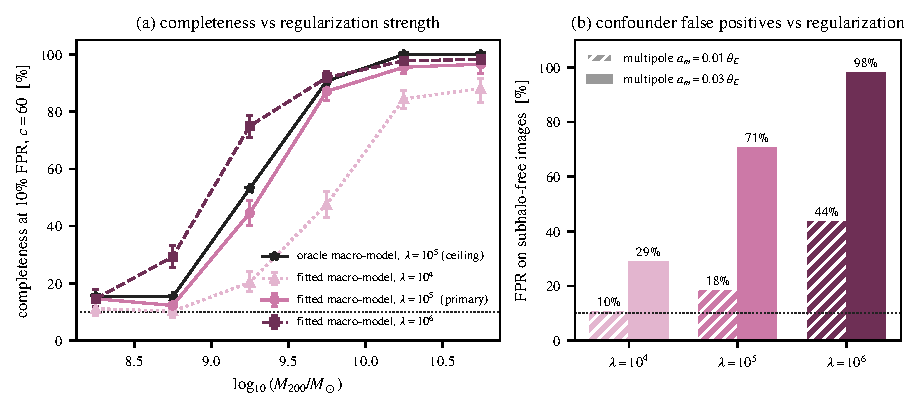
\includegraphics[width=\textwidth]{figures/fig8_family_b.pdf}
\caption{The free-form residual statistic's one free choice, the regularization strength $\lambda$. (a) Completeness at $c=60$ on the full 1\,000-lens populations for the fitted macro-model at three $\lambda$ ($10^{5}$ is the value used throughout; 68\% Wilson intervals) and, on the 300-lens seed-0 subsample, for the exact macro-model at $\lambda=10^{5}$ (black stars, the ceiling at that $\lambda$; a fitted curve at another $\lambda$ can exceed it). $\lambda=10^{4}$, $10^{5}$ and $10^{6}$ in light to dark shades of one hue. At $\lambda=10^{4}$ the statistic is dominated by fitted noise and its low-mass points scatter about the 10\% chance line; a point below the line is a fluctuation. (b) False-positive rate on the two multipole populations at the same three $\lambda$ (hatched: $a_m/\thetaE=0.01$).}
\label{fig:familyb}
\end{figure}

\clearpage

\begin{figure}[!htbp]
\centering
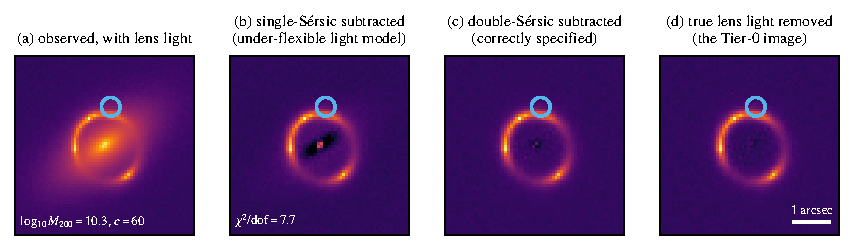
\includegraphics[width=0.82\textwidth]{figures/fig11_lenslight.pdf}
\caption{What lens light does to the image a detector sees. One $c=60$ subhalo lens: (a) as observed; (b) after subtracting the single S\'ersic fitted jointly with the mass model, whose misfit leaves a central residual brighter than any subhalo signature; (c) after the correctly specified double S\'ersic; (d) with the true lens light removed. The circle marks the true subhalo. Same arcsinh stretch throughout.}
\label{fig:lenslight}
\end{figure}

\clearpage
\begin{figure}[!htbp]
\centering
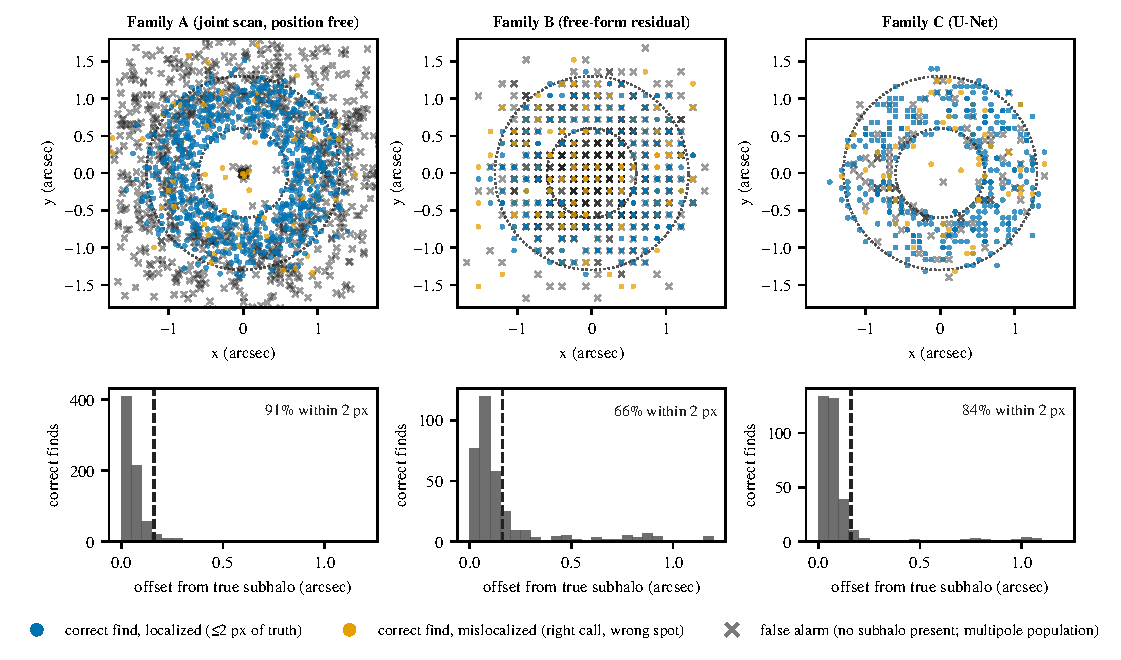
\includegraphics[width=\textwidth]{figures/fig4_localization.pdf}
\caption{Where each method points ($c=60$ population; the joint scan with the perturber position free, the free-form statistic and the U-Net seed~0), for the detections at each family's own 10\% threshold. Top: the reported position of every detection, blue if within 2~pixels ($0.16''$) of the true subhalo, orange if not; grey $\times$: false alarms on the multipole population; dotted rings: the placement annulus. Bottom: offsets of the correct finds, with the 2-pixel criterion dashed. Fractions are for each family's full detection sample; supplementary Table~S6 compares them on the common set.}
\label{fig:localization}
\end{figure}

\clearpage
\bibliographystyle{aa}\bibliography{refs}
\end{document}
